	\PassOptionsToPackage{brazil,american}{babel}
\documentclass[12pt]{article}

\usepackage{sbc-template}
\usepackage[brazil,american]{babel}
\usepackage[utf8]{inputenc}

\usepackage{graphicx}
\usepackage{url}
\usepackage{float}
\usepackage{listings}	
\usepackage{color}
\usepackage{todonotes}
\usepackage{algorithmic}
\usepackage{algorithm}
\usepackage{hyperref}

\sloppy

\title{Experimento 9\\ 
	FLIP-FLOPS:"T" E "D"}

\author{
	Lucas Mafra Chagas, 12/0126443 \\
	Marcelo Giordano Martins Costa de Oliveira,  12/0037301
}


\address{Dep. Ciência da Computação -- Universidade de Brasília (UnB)\\
	CiC 116351 - Circuistos Digitais - Turma C
	\email{\{giordano.marcelo, chagas.lucas.mafra\}@gmail.com}
}

\begin{document} 

\maketitle

 \begin{abstract}
	 In this experiment, we will study some types of flip-flops T and D by implementing, verifying their truth tables and comparing with the theoretical well-known results.
 \end{abstract}
     
 \begin{resumo} 
	 Neste experimento, serão estudados os alguns tipos de flip-flops T e D, através de sua implementação e posterior verificação de suas respectivas tabelas verdade, comparando-as com os resultados esperados teoricamente.
 \end{resumo}


\section{Objetivos}
\label{sec:Objetivos}

Descrição e implementação de flip-flops “T” e “D” usando portas lógicas ou flip-flops JK. Construção de flip-flops D gatilhado por nível ou pela borda usando portas lógicas; análise na transição de subida e descida do pulso de relógio. Aplicação dos flip-flops no projeto de um detector de sentido de movimento de um veículo.

\section{Materiais} 
\label{sec:Materiais}

\begin{itemize}
    \item Painel Digital
    
    \item \textit{protoboard}
    
    \item Fios
    
    \item Portas NAND, NOR, NOT, 2xFLIP-FLOP “D” (7474).
    
\end{itemize}


\section{Introdução}
\label{sec:Introducao}

O flip-flop T é um tipo de flip-flop que possui apenas uma entrada: a entrada de toggle T. Sempre que mudamos o estado de T, temos que a saída sofrerá modificação e irá para o seu estado inverso. Quando T possui um valor baixo, a saída permanece com o valor que possuia antes. Quando T possui um valor alto, a saída passa a ser o inverso do que era anteriormente. Temos, portanto, que a tabela verdade deste circuito é da seguinte forma: 

\begin{figure}[H]
	\centering
	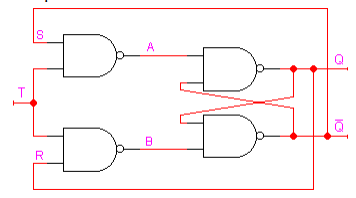
\includegraphics[width=.5\textwidth]{flipflopnand.png}
	\caption{Flip-flop T implementado com portas NAND}
	\label{fig:flipflopt}
\end{figure}

\begin{table}[H]
	\centering
	\begin{tabular}{|c|c|}
		\cline{1-2}
		\multicolumn{1}{|c|}{T} & \multicolumn{1}{|c|}{Qn+1} \\
		\hline
		0 & Qn \\
		\hline
		1 & $\overline{Qn}$\\
		\hline
	\end{tabular}
	
\end{table} 


Vemos no circuito que as mudanças de estado de S e R se propagam por 3 portas até chegar nas saídas. Portanto, temos que T precisa ter um pulso de no mínimo 20ns para que a reversão de estado no flip-flop seja garantida. Portanto, temos que a entrada T precisa entrar no circuito conectada à seguinte estrutura:

\begin{figure}[H]
	\centering
	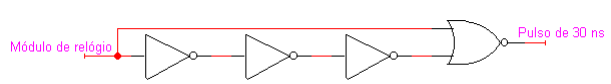
\includegraphics[width=.5\textwidth]{pulso.png}
	\caption{Produção de pulsos com duração de aproximadamente 30 ns}
	\label{fig:pulso}
\end{figure}

Dessa forma evitamos o estado de indeterminação e o flip-flop funcionará corretamente.
O flip-flop D é um flip-flop que possui uma entrada e um Clock. Essa entrada é diretamente ligada à saída. Portanto, quando mudamos o Clock, independentemente do valor atual que a saída possui, ela irá se ajustar para corresponder ao valor de D. Para este flip-flop, temos que a informação é incluída na saída um ciclo depois de ela ter chegado na entrada.
Fazendo a comparação deste flip-flop com um flip-flop RS gatilhado, temos que este flip-flop nunca terá a mesma entrada para SET e RESET, pois temos que SET recebe D e RESET recebe D. As figuras abaixo ilustram o circuito e o funcionamento deste flip-flop:

\begin{figure}[H]
	\centering
	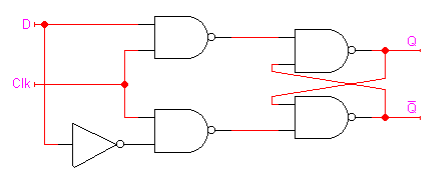
\includegraphics[width=.5\textwidth]{flipflopdgatilhado.png}
	\caption{Flip-flop D gatilhado por nível}
	\label{fig:flipflopd}
\end{figure}

\begin{table}[H]
	\centering
	\begin{tabular}{|c|c|c|}
		\cline{1-3}
		\multicolumn{1}{|c|}{Clk} & \multicolumn{1}{|c|}{D} & \multicolumn{1}{|c|}{Qn+1} \\
		\hline
		0 & 0 & Qn \\
		\hline
		0 & 1 & Qn \\
		\hline
		1 & 0 & 0 \\
		\hline
		1 & 1 & 1 \\
		\hline
	\end{tabular}
	
\end{table} 

\begin{table}[H]
	\centering
	\begin{tabular}{|c|c|}
		\cline{1-2}
		\multicolumn{1}{|c|}{D} & \multicolumn{1}{|c|}{Qn+1} \\
		\hline
		0 & 0 \\
		\hline
		1 & 1\\
		\hline
	\end{tabular}
	
\end{table} 


Temos que este flip-flop D tem sua saída modificada apenas quando o Clock é 1. Porém, é possível construir um flip-flop D gatilhado pela borda que permite que a entrada seja modificada ainda quando há a mudança de pulso, de 0 para 1. A imagem abaixo apresenta as características deste flip-flop:


\begin{figure}[H]
	\centering
	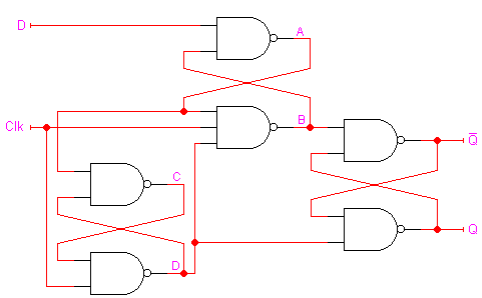
\includegraphics[width=.5\textwidth]{flipflopdnand.png}
	\caption{Implementação de um flip-flop D gatilhado pela borda positiva com portas NAND}
	\label{fig:flipflpodnand}
\end{figure}

\begin{table}[H]
	\centering
	\begin{tabular}{|c|c|c|}
		\cline{1-3}
		\multicolumn{1}{|c|}{Clk} & \multicolumn{1}{|c|}{D} & \multicolumn{1}{|c|}{Qn+1} \\
		\hline
		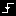
\includegraphics[width=.05\textwidth]{opa.png} & X & Qn \\
		\hline
		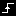
\includegraphics[width=.05\textwidth]{opa2.png} & 0 & 0 \\
		\hline
		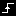
\includegraphics[width=.05\textwidth]{opa2.png} & 1 & 1 \\
		\hline
	\end{tabular}
	
\end{table} 

Este flip-flop é gatilhado pela borda positiva, porém, é possível construir um flip-flop gatilhado pela borda negativa, onde a mudança de estado irá ocorrer quando o pulso vai de 1 para 0.
É possível construir um todos os flip-flops mencionados acima a partir de um flip-flop JK. Para transformar um flip-flop JK em um flip-flop RS apenas conectamos S a J e R a K. Porém, teremos que evitar, para este caso, o estado 11. Para transformar um flip-flop JK em um flip-flop D, é necessário apenas incluir um inversor entre os terminais J e K. Para transformá-lo em um flip-flop T, considera-se que as entradas J e K são ambas T De tal forma, T irá definir se aceita ou não o pulso enviado pelo relógio.
Ao lidar com flip-flops é necessário sempre considerar uma propriedade importante: o tempo de setup do flip-flop. O tempo de setup de um flip-flop é definido como o menor intervalo de tempo em que o sinal da(s) entrada(s) deve(m) estar já no nível correto e ser(em) mantido(s) antes da ocorrência de uma transição no relógio.  Para a família TTL esse tempo é de 20ns.

\section{Procedimentos}
\label{sec:Procedimentos}

Neste experimento, faremos a construção dos flip-flops mencionados acima e analisaremos o seu funcionamento.

\subsection{Montar um flip-flop “T” utilizando apenas portas NAND.}
\label{2.1}
Para esta parte do experimento foi montado um circuito de acordo com o esquema apresentado na figura abaixo:

\begin{figure}[H]
	\centering
	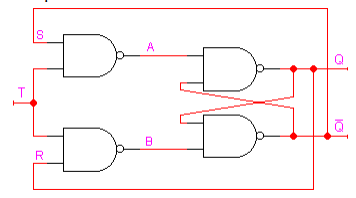
\includegraphics[width=.5\textwidth]{flipflopnand.png}
	\caption{Flip-flop T implementado com portas NAND}
	\label{fig:flipfloptexp}
\end{figure}	

Além disso, para respeitar o tempo de mudança de estado e as saídas  e  apresentarem os valores corretos após um pulso de  foi montado um circuito auxiliar que fazia com que a duração de  fosse de no mínimo 30ns (tempo necessário para se alterar  e  devido ao números de portas lógicas na qual a mudança deve se propagar). O esquema desse circuito encontra-se na figura abaixo:

\begin{figure}[H]
	\centering
	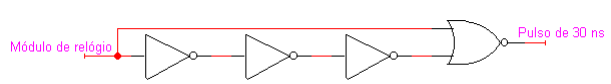
\includegraphics[width=.5\textwidth]{pulso.png}
	\caption{Produção de pulsos com duração de aproximadamente 30 ns}
	\label{fig:pulsoexp}
\end{figure}

Após a construção do circuito, fez-se a análise dos resultados para a obtenção da sua tabela verdade. Depois disso, inserindo a entrada de  em um gerador de frequências de 1 Hz criou-se um diagrama de frequências para este flip-flop.


\subsection{Montar um flip-flop “D” gatilhado por nível.}
\label{2.2}

Fez-se, construiu-se um flip-flop “D” gatilhado por nível, como mostra o esquema na figura abaixo:

\begin{figure}[H]
	\centering
	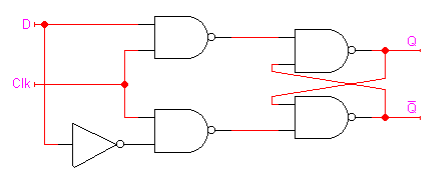
\includegraphics[width=.5\textwidth]{flipflopdgatilhado.png}
	\caption{Flip-flop D gatilhado por nível}
	\label{fig:flipflopdexp}
\end{figure}

Depois da implementação obteve-se a tabela verdade desse circuito.

\subsection{Montar um flip-flop “D” gatilhado pela borda.}
\label{2.3}

Como na parte 2.2., construiu-se o circuito a partir de um esquema, fez-se a obtenção da sua tabela verdade e observou-se o seu comportamento ao aplicarmos um pulso no Clock. O circuito montado e o seu esquema encontram-se nas figuras abaixo:

\begin{figure}[H]
	\centering
	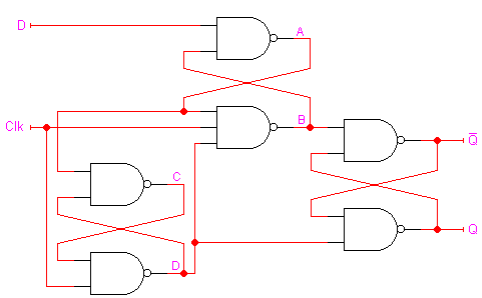
\includegraphics[width=.5\textwidth]{flipflopdnand.png}
	\caption{Implementação de um flip-flop D gatilhado pela borda positiva com portas NAND}
	\label{fig:flipflpodnandexp}
\end{figure}



\subsection{Montar, verificar e explicar o funcionamento de um flip-flop “D” com circuito auxiliar de produção de pulsos.}
\label{2.4}

Utilizando-se o circuito montado em 2.3., adicionou-se à entrada um circuito auxiliar de produção de pulsos, como mostra a figura abaixo:


\begin{figure}[H]
	\centering
	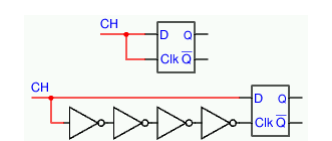
\includegraphics[width=.5\textwidth]{auxiliarpulso.png}
	\caption{Circuito auxiliar de produção de pulsos}
	\label{fig:auxiliarpulsoexp}
\end{figure}

Observou-se então o funcionamento do circuito após a inclusão deste circuito auxiliar.

\subsection{Projetar um circuito sequencial que detecta o sentido de movimento de veículos em uma rua.}
\label{2.5}

\begin{figure}[H]
	\centering
	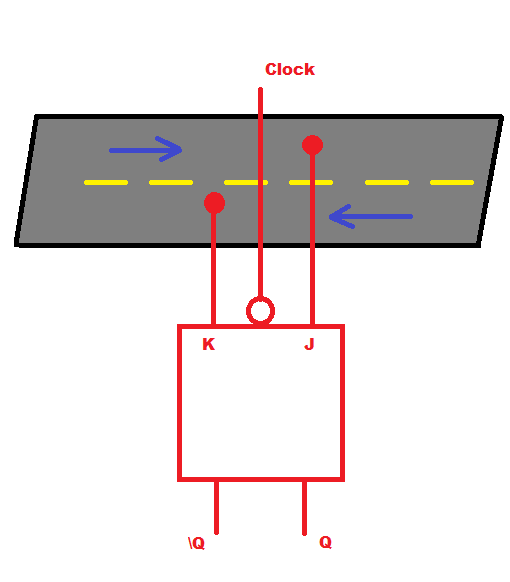
\includegraphics[width=.5\textwidth]{desafiocarro.png}
	\caption{Circuito sequencial que detecta o movimento de veículos construído com um flip flop JK}
	\label{fig:desafiocarroexp}
\end{figure}

Este circuito, como especificado, possui apenas 2 entradas e duas saídas. Temos que se um carro vier da direita para a esquerda ele acionará o clock e em seguida acionará a entrada J. De tal forma, teremos Q = 1  e Q = 0. Se o carro vier da esquerda para a direita ele acionará o clock e ficaremos com Q = 0 e Q = 1. Quando o carro seguir em frente e desligar o clock o flip-flop irá armazenar a última informação incluída e, consequentemente, saberemos que quando Q = 1 o carro veio da direita. Quando Q = 0 o carro veio da esquerda. 



\section{Análise dos Resultados}
\label{sec:Resultados}

\subsection{Montar um flip-flop “T” utilizando apenas portas NAND.}
Após a implementação do circuito, foi verificado o que acontecia com a saída Q após a mudança do valor de T. O circuito foi iniciado com  Q = 0 e Q = 1. 

De acordo com as figuras e a análise feita em laboratório, obteve-se a seguinte tabela verdade:


\begin{table}[H]
	\centering
	\begin{tabular}{|c|c|}
		\cline{1-2}
		\multicolumn{1}{|c|}{T} & \multicolumn{1}{|c|}{Qn+1} \\
		\hline
		0 & 0 \\
		\hline
		1 & 0\\
		\hline
		0 & 1\\
		\hline
	\end{tabular}
	
\end{table} 

Generalizando essa tabela, ficamos com:

\begin{table}[H]
	\centering
	\begin{tabular}{|c|c|}
		\cline{1-2}
		\multicolumn{1}{|c|}{T} & \multicolumn{1}{|c|}{Qn+1} \\
		\hline
		0 & Qn \\
		\hline
		1 & Qn\\
		\hline
		0 & $\overline{Qn}$\\
		\hline
	\end{tabular}
	
\end{table} 

Observamos que essa tabela corresponde com o esperado: a saída Q se altera apenas após um pulso completo de T, com T indo de 0 para 1 e de 1 para 0 novamente. Inserindo um pulso de 1 Hz na entrada T, foi possível criar o seguinte diagrama de frequências:

\begin{figure}[H]
	\centering
	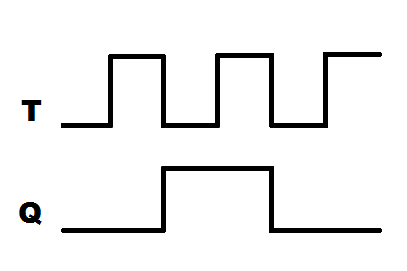
\includegraphics[width=.5\textwidth]{diagramat.png}
	\caption{Diagrama de frequências do um flip-flop “T” construído}
	\label{fig:diagramat}
\end{figure}

A partir do diagrama vemos que a saída Q é modificada na a cada duas transiçoes de T, ou seja, temos o esperado: a mudança de frequência de T é duas vezes mais rápida que a mudança de frequência de Q.

\subsection{Montar um flip-flop “D” gatilhado por nível.}

Fazendo a tabela verdade correspondente aos valores obtidos, temos que:

\begin{table}[H]
	\centering
	\begin{tabular}{|c|c|c|}
		\cline{1-3}
		\multicolumn{1}{|c|}{Clk} & \multicolumn{1}{|c|}{D} & \multicolumn{1}{|c|}{Qn+1} \\
		\hline
		0 & 0 & 0 \\
		\hline
		0 & 1 & 0 \\
		\hline
		1 & 0 & 0 \\
		\hline
		1 & 1 & 1 \\
		\hline
		0 & 0 & 1 \\
		\hline
	\end{tabular}
\end{table}

Generalizando esta tabela, ficamos com:

\begin{table}[H]
	\centering
	\begin{tabular}{|c|c|c|}
		\cline{1-3}
		\multicolumn{1}{|c|}{Clk} & \multicolumn{1}{|c|}{D} & \multicolumn{1}{|c|}{Qn+1} \\
		\hline
		0 & 0 & Qn \\
		\hline
		0 & 1 & Qn \\
		\hline
		1 & 0 & 0 \\
		\hline
		1 & 1 & 1 \\
		\hline
	\end{tabular}
\end{table}

Para este circuito temos o seguinte diagrama de frequências para o estado inicial Qn = 0:

\begin{figure}[H]
	\centering
	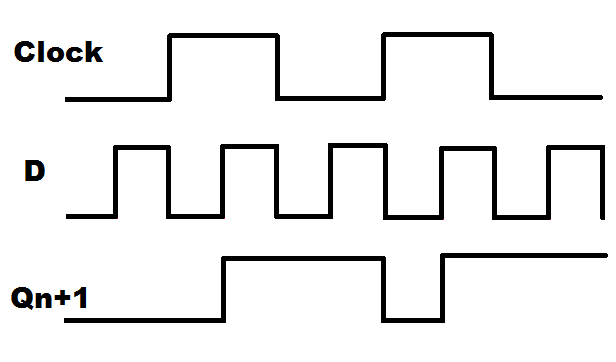
\includegraphics[width=.5\textwidth]{diagramad.png}
	\caption{Diagrama de frequências para o flip-flop “D” construído}
	\label{fig:diagramad}
\end{figure}

\subsection{Montar um flip-flop “D” gatilhado pela borda.}

Feita a implementação do flip-flop apresentado na Figura 6, observou-se o comportamento do circuito.

A partir do experimento e sabendo que o valor inicial de  era 0, podemos montar a seguinte tabela verdade para este circuito:

\begin{table}[H]
	\centering
	\begin{tabular}{|c|c|c|}
		\cline{1-3}
		\multicolumn{1}{|c|}{Clk} & \multicolumn{1}{|c|}{D} & \multicolumn{1}{|c|}{Qn+1} \\
		\hline
		0 & X & 0 \\
		\hline
		0 $\rightarrow$ 1 & 0 & 0 \\
		\hline
		1 $\rightarrow$ 0 & X & 0 \\
		\hline
		0 $\rightarrow$ 1 & 1 & 1 \\
		\hline
		1 $\rightarrow$ 0 & X & 1 \\
		\hline
		0 & 1 & 1 \\
		\hline
	\end{tabular}
\end{table}

Generalizando esta tabela, ficamos com:

\begin{table}[H]
	\centering
	\begin{tabular}{|c|c|c|}
		\cline{1-3}
		\multicolumn{1}{|c|}{Clk} & \multicolumn{1}{|c|}{D} & \multicolumn{1}{|c|}{Qn+1} \\
		\hline
		1 $\rightarrow$ 0 & X & Qn \\
		\hline
		0 $\rightarrow$ 1 & 0 & 0 \\
		\hline
		0 $\rightarrow$ 1 & 1 & 1 \\
		\hline
	\end{tabular}
\end{table}

Vemos, a partir da generalização da tabela do circuito montado, que ele está correto, correspondendo com o resultado teórico (que era o resultado esperado). Fazendo o diagrama de frequências para este circuito ficamos com:

\begin{figure}[H]
	\centering
	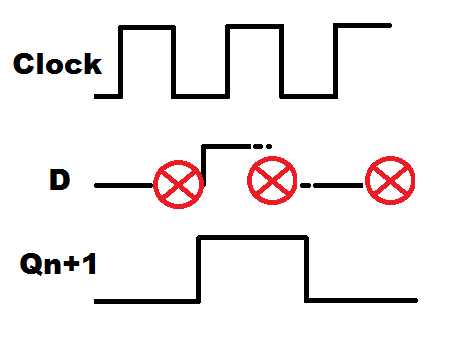
\includegraphics[width=.5\textwidth]{diagramadgatilho.png}
	\caption{Diagrama de frequências para o flip-flop construído em 2.3 (obs.: o X vermelho está representando o fato de que não importa o valor de , pois nesse instante temos o Clock indo de 1 para 0)}
	\label{fig:diagramadgatilho}
\end{figure}


\subsection{Montar, verificar e explicar o funcionamento de um flip-flop “D” com circuito auxiliar de produção de pulsos.}

O circuito de 2.3 foi incrementado com o circuito auxiliar de produção de pulsos para gerar o circuito desenvolvido. 

Aqui, a entrada D e a entrada de Clock tinham origem em um mesmo ponto, a chave A. Porém, essa entrada foi dividida em duas e o Clock passou por 4 portas NAND antes de chegar em suas portas de destino, gerando portanto, um atraso de 40ns em relação à entrada D. Temos que esse circuito não funcionou adequadamente, com a saída tendo o valor esperado em certos momentos e em outros não.  Isso ocorreu pois o tempo de setup do circuito não estava sendo respeitado. Temos que nesse circuito existem portas que dependem diretamente do resultado de D e do resultado do Clock sendo inseridos ao mesmo tempo, e, portanto, com o atraso de propagação, obteve-se um erro no resultado. Esse ajuste provavelmente teria sido benéfico caso ele fosse inserido em um flip-flop “D” não gatilhado.


\section{Conclusão}
\label{sec:Conclusao}

Com este experimento foi possível observar o funcionamento de flip-flops “T” e “D” devido ao sucesso na construção dos circuitos de cada uma das partes. Foi possível compreender o funcionamento de mais dois tipos de flip-flop e analisar o seu relacionamento com os flip-flops previamente estudados. Além disso, foi possível ver (graças à parte 2.5.) momentos em que estes flip-flops poderiam ser implementados no nosso dia a dia.

\newpage 
% Colocar aqui apenas as respostas dos itens da Auto-Avaliação
\section*{Auto-Avaliação}

\begin{enumerate}
    \item B
    \item C
    \item A
    \item C
    \item C
    \item E
    \item C
    \item B
    \item B
    \item A
\end{enumerate}


\end{document}
